%************************************************
\chapter{Use of a Middleware Layer with Ontologies}\label{ch:middleware}
%************************************************
\section{Introduction}\label{sec:mwintro}
The benefits of adopting linked data and related techniques, even in environments with substantial legacy resources are clear. In essence this is achieved by first modelling the schema of the data, then making the ABox (row) data available to the ontology. Once an area or sub-domain has been modelled, software must be developed that allows software and services within the industry to interact with the the data in the triple store. This currently requires specialist knowledge, not common in the software engineering community, and this gap presents another barrier to industrial implementation of ontology based systems. As a minimum a developer working in the area would need a detailed understanding of:
\begin{itemize}
    \item SPARQL;
    \item XML data types;
    \item The APIs for the triple store to be used.
\end{itemize}

In addition to these, for the knowledge of the specific technologies to be of value, a certain amount knowledge of higher level ontology principles is required. At the very least a familiarity with triples and, in an environment where reasoning is used, inference is also required. It is reasonable to expect that most professional software engineer will have some knowledge of XML data types, on that basis it should be possible for them to learn the basics required to interact with the triplestore within the lifespan of any large industrial project, learning SPARQL or higher level concepts will take significantly longer.

Whilst it is likely that in the long term the skills gap around ontology will be filled by improved education and training in the short and medium term the adoption of ontology linked data in the rail domain would be considerably accelerated by the production of tools that enable software engineers without ontology experience to interact with data stored using an ontology. The RaCoOn middleware exists to bridge that gap.

\subsection{Questions Considered}

This chapter will make it possible to consider the following questions, posed in \autoref{ch:probstate}:
\begin{itemize}
\item \QuestionCombine
\item \QuestionChange
\item \QuestionSkillz
\end{itemize}

\subsection{Roles}
The RaCoOn middleware exists as an intermediary between the triple store holding the ontologies, and applications that require access to those resources. In addition to enabling this simple connectivity the middleware also provides and manages connections to REDIS, a key value store used to handle high frequency data, and adds a security layer. Applications use the middleware via Windows Communication Foundation (WCF) web services, which where ever possible implement RESTFul design principles. The middleware represents several contributions to ontology development for the railways: Firstly it acts as a \say{buffer} between the triple store and the connected applications (consumers). Different consumers have a range of access requirements and as the market evolves it is possible, even likely, that the selection of commercially available triple stores will change. The middleware ensures that as the software components on either side of the middleware evolve the larger system is unaffected; the same interface will be presented to the consumer regardless of the choice of triple store. Another key benefit the use of a middleware offers, is the ability for developers to easily interact with a range of specialist datastores as needed by the application use case alongside the triplestore itself. In the scope of this document, this is illustrated using the REDIS key-value store as a lookup for high frequency data streams, however, as the technology develops many other similar storage needs are likely to be identified.

Since some data stores don't have their own security, an additional benefit of the middleware is a single sign on and token system can be handled by the middleware.After a user is authenticated by the middleware and given a token allowing continued access all datastores behind the middleware are accessed using that token, regardless of the security mechanism they employ. For systems that have complex access control hierarchies it is possible to map each user signing on to the middleware to their unique username, whilst systems bereft of security can be shielded from outside access. 

By using a middleware common functions shared by a number of applications can be implemented at this level avoiding duplication. The WCF webservices make it possible to connect to the middleware using clients written in most common languages and from most environments, allowing developers to use the best tool for the current project. The overall architecture is summarised in \autoref{fig:MiddlewareHL}.

\subsection{Data Volumes}

A major challenge to the migration from the current ecosystem of mixed incompatible data stores to one that embraces linked data and ontology, is that of data volumes. Whilst the market for triple stores has moved forward significantly in the last five years and a number of triple stores will now scale to significant volumes of data when run in an appropriate environment, triples are an inherently inefficient way to store most types of data. High frequency data streams, which are common in industrial applications, such as remote condition monitoring, are particularly difficult to handle in most triple stores due to the computational overhead associated with rapid updates. \citet{Tutcher2015} mitigated this problem by supplementing the triple store with REDIS, which acted as a buffer for the high frequency data.

The triple store holds a summary of the data along with a link which can be used to retrieve it from another store. For example where a complex wave form is recorded, its amplitude, duration and the time at which the sample was taken could be stored as triples, alongside a key to retrieve it from REDIS. REDIS is highly optimised for fast retrieval of large amounts of data using a very simple key, deliberately leaving security entirely to the user.

 \begin{figure}[H]
\myfloatalign
{\includegraphics[width=\linewidth]{gfx/Middleware_role}} 
\caption{The role of the Middleware}
\label{fig:MiddlewareRole}
\end{figure}

\section{Functionality}
 \label{sec:function}
For the middleware to provide the services shown in \autoref{fig:MiddlewareRole} it must provide a number of functions:
\begin{itemize} 
    \item Brokering: acting as an intermediary between client and server;
    \item Datastore aggregation;
    \item Provision of stored procedures;
    \item Provision of datastore security;
    \item Provision of common functionality.
\end{itemize}

Each of these will be discussed in the following sections.

\subsection {Brokering: acting as an intermediary between client and server}
The middleware must act as a broker or intermediary between applications consuming and contributing to datastores. One of the challenges the industry will face during a transition to linked data is that as the datastores available evolve with time, and new technologies are developed the interfaces the datastores present will also change.

In an established industry it can be expected that new client applications will be created on an as needed basis when required for a project. This will likely be over an extended period, probably measured in years and there will be no \say{big bang} style switch-over event in which the entire industry is migrated over to linked data over night. 

Suppliers are starting to respond to the industrial need for easier to use interfaces to triple stores, and SPARQL has existed as a constantly evolving standard query language for some time; however this alone does not alleviate the risks of vendor lock in when choosing a triple store, and thus the provision of intermediaries between the data store and the end user applications is certainly prudent, if not necessary.

\subsection{Datastore aggregation}
New datastores are being developed rapidly as the technology matures, all with different strengths and weaknesses. As the market evolves it is possible, even probable, that new railway projects will require access to different types of data store, in keeping with the project's needs. In the first instance REDIS has been selected as a second data store to make available, since this has been used in previous projects with RaCoOn for high frequency data. Many railway condition monitoring applications, such as alternating current field measurement sensors to detect cracks in rails, or laser distance sensors, as used in condition monitoring of railway assets can generate very high volumes of data.
\subsection{Stored Procedures}
The middleware provides \say{Stored Procedure} functionality similar to that commonly found in relational databases. This has several benefits, applicable to both relational data stores and this system:

\begin{itemize}
    \item Improved reuse. Once a stored procure has been written it can be used by many systems, or the same system in many places with out rewriting it;
   \item Isolation between the software and the query. As such if the representation of the data changes only the query need change, not the system using it. In the case of ontologies, as opposed to relational databases, this should only be relevant if major re-factoring is done for example if a different domain had to be used for all URI's in the system.
    \item Familiarity for developers used to a relational database environment;    
    \item Less data needs be sent to the middleware since the name of the stored procedure is much shorter than the SPARQL required to describe the query. 
\end{itemize}

By providing a familiar mechanism to developers coming from a relational database background, the middleware reduces the learning curve for those new to the technology. Other benefits from the relational database domain are less applicable to the linked data domain, in particular the stored procedures can't be pre-compiled for faster execution, since the middleware is not responsible for the compilation of the query.

Stored procedures created in the middleware can seamlessly use any datastore, there is no difference to the user and no changes to the implementation need be made when a different store is used, though it is likely that the stored procedure will need to be updated to match the API provided by the new store. Application code which has been developed to use one data store via the middleware will continue to do so transparently when another is added. 


\subsection{Information Security}
Information Security has become an important research topic recently, as the possibilities of electronic crime and attacks against infrastructure are considered.

The question of information security is a broad topic, and it is beyond the scope of this thesis to address it in its entirety. It is however necessary to investigate the impact on information security of moving to a system of linked data and ontology.
It is common in the literature to divide information security challenges into three areas: 
\begin{description}
    \item[Confidentiality] Presenting the improper disclosure of information as considered by \citep{Erlingsson2016};
    \item[Integrity] Insuring that information remains accurate;
    \item[Availability] Ensuring that information remains available in all circumstances. 
\end{description}

Triple stores are reaching a level of maturity similar to that of relational databases, this includes the ability to cluster for both improved scalability and availability. Running triple stores in a virtualised cloud environment can also result in increased availability of data. 

When considering information integrity, ontology allows the insertion of provenance information, making it possible to understand why any given change was made to the data. Whilst it has not be implemented, in this work, at the middleware level it should be possible to include functionality in the middleware to automatically append provenance to data as it was inserted. 

The most significant contribution the use of the middleware makes to information security can be found in confidentially. By imposing a secure layer between the unsecured data store and the wider network (or indeed internet) the middleware prevents unauthorised access to other datastores. Taken in conjunction with the datastore aggregation this approach has the added advantage of providing a ``single~sign~on'' for all datastores. The trusted component, in this case the middleware, is accessible from client machines however all hosts running datastores trust \textbf{only} the middleware and not the larger network. 

\subsection{Centralising Common Functionality}\label{midfunc}
In an ontology architecture using middleware common functionality may be moved into the middleware to avoid needless repetition in keeping with the software development doctrine of \say{Don't Repeat Yourself (DRY)}. This centralisation of functionality can make clients lighter weight and less time consuming to develop. The middleware must also implement functionality to handle security and to query the data stores the middleware connects to, both using stored procedures and queries. The following functionality is commonly needed by systems connected using an ontology for data storage:
\begin{itemize}
    \item Free text search of individuals within a class, using the label text;
    \item Get all individuals of a given type;
    \item Add new items.    
\end{itemize}


\section{Middleware Design Patterns}
When developing an ontology architecture the techniques used to link client applications to datastores are similar to those faced in any other domain of software engineering. 
The design of this software employed several common software engineering techniques for example, where exactly one instance of a class was required, such as connecting to a datastore, the \say{Singleton} pattern was employed to ensure only one instance was ever created. Additionally in order as to prevent repetition of code SOLID principles (previously discussed in \autoref{ch:cifparser}) were employed.

\section{Implementation}
In order as to provide the functionality set out in \autoref{sec:function}, the middleware was implemented as collection of webservices, using the windows communication foundation (WCF). These can be consumed by clients created using a range of development techniques, and libraries exist to aid connection to WCF webservices from several languages, however it is most common to use the .Net family of languages for the client.

\subsection{Modular Structure}
The middleware solution contains the following modules:
\begin{description}
    \item[RacoonMiddleware] Holds the Webservices and calls the other projects as needed;
    \item[MiddlewareBussinessObjects] Holds representations of objects referred to by the ontology as C\# objects;     
    \item[REDISConnector] Acts as the intermediary between the middleware and REDIS.
    \item[StoredProcCreator]
    This module compiles to provide a simple graphical (Win32) interface for creating and editing stored procedures. 
    \item[StardogConnection]  Acts as the intermediary between the middleware and Stardog.    
    \item[UploadLDLTool]
    This module compiles to a very simple graphical tool (Win32) for testing the processing of LDL files, required for a specific project which is set out in  \autoref{ch:COMPASS}. It is not intended for production use, rather it was a debugging tool before the functionality had been added to another system.
    \item[UserManager]
    This tool manages the users that have access to the middleware. It is a small, simple tool for use by system administrators.
\end{description}

The relationship between these modules and external modules is shown in \autoref{fig:MiddlewareHL}.

\begin{sidewaysfigure}
\myfloatalign
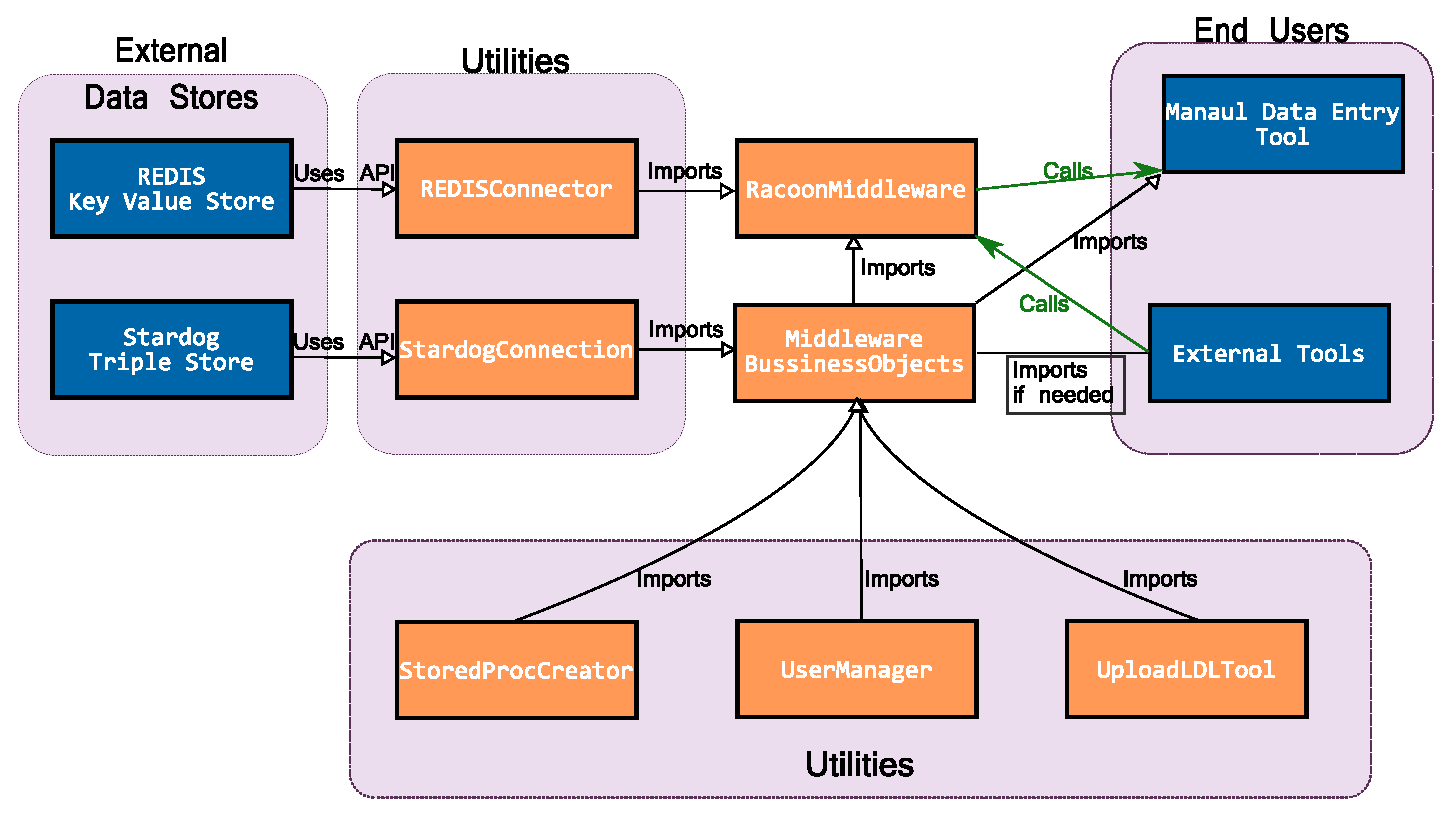
\includegraphics[max height=0.9\textwidth]{gfx/MiddlewareHighLevel}
\caption{The interactions between the middleware modules, both internal and external}
\label{fig:MiddlewareHL}
\end{sidewaysfigure}

\subsection{RacoonMiddleware}
\label{sec:middlewaremodule}
This module contains the webservice definitions and the functionality directly related to them and thus is the part of the middleware with which external developers will interact directly. In particular it contains definitions of all the responses that can be given by the webservices and all the parameters accepted.

In keeping with software engineering best practice, for systems providing many similar functions, this module in particular makes heavy use of SOLID design patterns. \\ All of the responses returned by the webservice extend a simple base class entitled \say{\texttt{SimpleRacoonResponse}}, which provides the basic details every response from the webservice will include, namely:
\begin{description}
    \item[AuthorisationOK] A Boolean value indicating if the token provided was accepted. If this is false then the token is not valid. The most probable cause for this is the token timing out, since they are only valid for a given length of time, currently configured as one hour.
    \item[Error] An exception, if this is not null an error of some kind has occurred. The message should be suitable for display to a user and the type of the exception should be informative.
    \item[Status] If this is true the operation completed successfully and the results can be replied upon. If it is false then the results should be discarded. 
\end{description}

This inheritance is set out in \autoref{fig:MiddlewareResponses}, which also gives details of the possible response types. The response classes in turn all either implement one of the interfaces set out in \autoref{fig:ResponseInterfaces} or a extend a class that does. This was in keeping with good object orientated design practice, since every response requires some common authorisation and error handling functionality as set out above and it allows the system both handling and generating those responses to be written once, not rewritten for every webservice.  Inheritance was also used by the classes implementing the webservices, in keeping with the principles of reusing code rather than copying it, as shown in \autoref{fig:services}.

\begin{sidewaysfigure}
\myfloatalign
{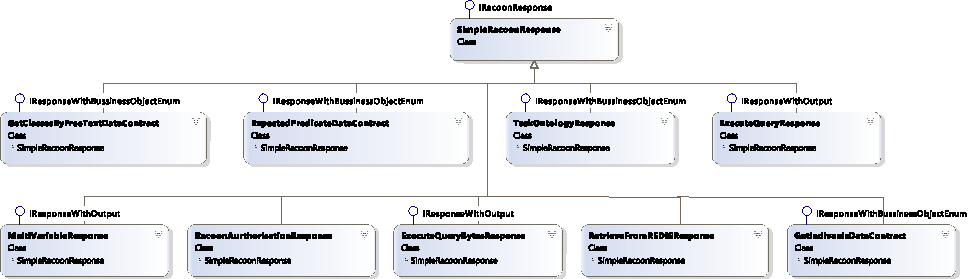
\includegraphics[width=\paperwidth]{gfx/MiddlewareServicesClassesResponseOnly}} 
\caption{The response types returned by the RaCoOn Middleware}
\label{fig:MiddlewareResponses}
\end{sidewaysfigure}

 \begin{figure}
\myfloatalign
{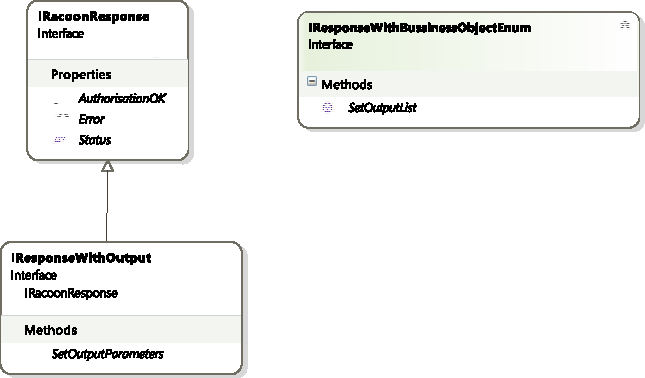
\includegraphics[width=\textwidth]{gfx/Res}} 
\caption{The interfaces implemented by webservice responses}
\label{fig:ResponseInterfaces}
\end{figure}

 \begin{sidewaysfigure}
\myfloatalign
{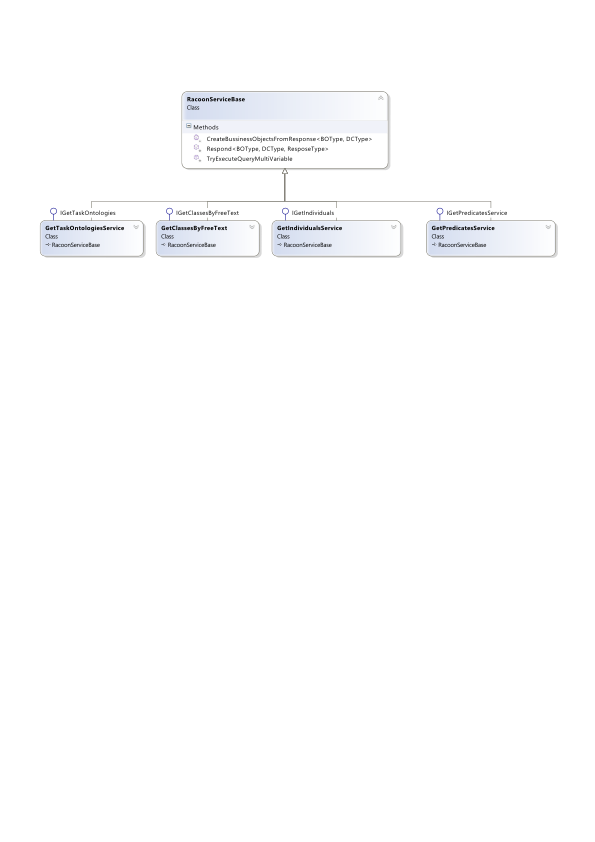
\includegraphics[width=\paperwidth]{gfx/RacoonServices}} 
\caption{Selected webservices}
\label{fig:services}
\end{sidewaysfigure}

The \texttt{RacoonMiddleware} module is also responsible for acting as an \say{intermediary} between multiple different data stores. Within the framework discussed Stardog is used as the main datastore (the triplestore), with REDIS support included to provide a buffer for high velocity data streams. However the framework is flexible and would allow for the addition of extra datastores with no impact on the existing stores or the framework. In order as to isolate this datastore specific code from the rest of the system it is implemented in separate Dynamic Link Libraries, here on referred to as DLLs. This allows for; the easy addition of new datastores, reduced regression testing when the DLL is changed to match changes in triple store interfaces and logical separation from unrelated code. In order as to be usable by the larger system the DLL must make available or \say{export} an implementation of the interface set out in \autoref{lst:query}. Stored procedures have a field setting out the fully qualified name of the stored procedure's type, as seen in \autoref{lst:StoredProcedure} so if the DLL is in memory all that needs be done to access a new datastore is create a stored procure with that type specified and it will be used, with no code changes to this module. 

\vfill
\begin{lstlisting}[language={[Sharp]C},frame=tb,caption={The IQuery interface, which must be implemented by all executable queries},label=lst:query]
/// <summary>
/// An abstract query, targeting any data store. Includes methods for setting any variables included in the query
/// </summary>
public interface IQuery
{
    void SetTarget(string server,string datastore);
    void SetQuerry(string queryText);
    IEnumerable<MiddlewareParameter> Execute(IEnumerable<MiddlewareParameter> parameters, Session session, ParameterTypeEnum returnTypeWanted);      
}
\end{lstlisting}

As can be seen from \autoref{lst:query} queries and stored procedures managed via the middleware can take any number of parameters, which can be one of several types:

\begin{description}
    \item[Uri]  Unique Resource Identifiers, as used in linked data;
    \item[String] String data and all other data types not specifically handled;    
    \item[Byte] For transferring binary data.
\end{description}

This list can be expanded if needed. These restrictions only apply to stored procedures and to functions directly passing queries. Task specific webservices can take or return any type including a business object related to the operation they perform, or a simple in built types.

This system of stored procedures can have a significant impact on the ease of integration of software systems. This also makes it possible to demonstrate how stored procedures can query multiple data stores. As such they are implemented within the  \texttt{RacoonMiddleware} module, \autoref{lst:StoredProcedure} shows the implementation.

An XML file, holding numerous instances of the class shown in The implementation of the stored procedures is included in \autoref{app:spList} in \autoref{lst:StoredProcedure} provides the database of stored procedures. For efficiency this is read into a dictionary in memory on start-up then stored procures are retrieved, using a hash of the stored procedure's name as its key in the dictionary. This allows for very fast access to stored procedures, which is necessary when dealing with high velocity data, such as that from sensors.

\subsection{MiddlewareBussinessObjects}
Modelling real world data in object orientated programming as \say{Business Objects} is a staple programming technique when dealing with conventional data storage. Typically the business objects either hold only instance data, in which case it is known as an \say{anaemic domain model}. The alternative, putting business logic and validation in the business objects is known as a \say{rich domain model}. Where ever the restrictions are placed, be they in the domain model or in another layer, this is where traditional developers model the domain. When using ontologies both the model and as much as possible of the business logic belong in the ontology, however, in order as to work with this in a conventional programming language business objects, repeating those in the ontology are required for all items the software has to interact with. For example, the ontology may have a very detailed model of a train and its components, however a passenger information application would not need (or want) a ``Wheel'' business object, trusting instead that the ontology presented the correct behaviour of a train service and modelling only that service concept in the application. 

Modelling concepts stored in an ontology as business objects in a programming language makes manipulating them more intuitive, both for external users and for developers working on the middleware. Frameworks exist that can automatically generate objects from classes held in triple stores\footnote{the open source module JENA has this capability}, however, at point this work was undertaken none were available for C\# and business object development was done manually. Note that whilst ontologies allow multiple inheritance neither C\# nor JAVA are able to support it. In the implementation for this system interfaces were used to address this issue, removing the need for inheritance from multiple base classes.

This entire module is compiled as a DLL, to allow for its reuse in other systems and to keep coupling between the business objects and the implementation of the webservices loose.
\subsubsection{From objects to individuals}
Moving from the ``Open World'' model common to RDF and ontologies, to the more familiar paradigms of Object Orientated languages requires developers (or the designer of the tool, where this is automated) to make some decisions as to how the classes and properties of the data model are modelled as objects and properties in the business objects. In the case of object properties, that is properties that \say{connect pairs of individuals} as specified in \citet{McGuinness04}, representation as an object is possible, so long as both the individuals to be linked are of types already modelled in the system. Unless there are cardinality restrictions, such as marking a property as functional, then using a list or similar collection class is an appropriate way to link objects, unless the developers domain knowledge rules out this possibility. For example when linking objects of type train and driver via an object property of type ``currentDriver'' it would be unnecessary to use a list, even if the property has not had any cardinality restrictions placed upon it to reduce the amount of reasoning required. This is illustrated in \autoref{lst:bgtob} which shows the relationship between Balises and Balise Groups. Cardinality restrictions require checking when an object is inserted and thus represent a (small) performance cost. In the most restrictive of decision logics cardinal restrictions are not available; if a property is marked as functional, that is it uses the type \texttt{owl:FunctionalProperty}, then an individual can have at most one value for that property. Rules will remain encoded in the ontology, rather than be duplicated in business objects, to allow changes to be made to the rules in the ontology.

\begin{lstlisting}[language={[Sharp]C},frame=tb,caption={Linking of Balises to BaliseGroups},label=lst:bgtob]
   public List<LDLBalise> Balises;
\end{lstlisting}

In an industrial environment characterised by legacy systems, business objects may also be used to model source data sets for insertion into the ontology. Whilst this seemingly extraneous step isn't required in every instance, where the data is complex it allows it to be normalised and collated before its insertion to the ontology.

In the case of \texttt{Datatype properties}, also known as value properties, all that need be done generally is adding a public field of the appropriate type to the object. The datatypes are restricted to inbuilt XML data types, which align with the available datatypes in most programming languages. 

\subsection{Datastore connections}
As discussed in \autoref{sec:middlewaremodule} a modular architecture is employed through this system. The modules which connect to external datastores are refereed internally, and by this document, as ``Connectors''. In the RaCoOn Middleware two modules, \texttt{Stardog Connector} and \texttt{REDIS Connector} are examples of means of connecting to external data stores. These are compiled as DLLs and so as they are loaded into memory when the software requires them. New connectors can be added with little or, in the case of stored procedures using only stored procedures, no alteration to the other modules. By implementing connectors, and hence decoupling the software artefacts using them, the danger of cascades of changes needing to be made in response to a change in one of the connectors is greatly reduced. Among the benefits of this is reduced regression testing when altering any given module. 

In order as to be used by the wider system the module exports a \texttt{Query}, compliant with the \texttt{IQuery} interface defined in \autoref{lst:query} allowing the RacoonMiddleware to query this data store.

\subsubsection{Stardog Connector}

The stardog connector module shows how a triple store can interact with the middleware and then client applications. The dependencies directly pertaining to stardog are imported in this module. Should they require updating (as they periodically do) then only this module requires recompilation.

\subsubsection{REDIS Connector}

This DLL has functionally related only to the REDIS key-value store. It exposes those of the APIs functions such as are required for use with an ontology architecture and maintains the required state information.

\subsection[Administration Tools]{Administration tools \\ Other Modules: StoredProcCreator, UploadLDLTool, and UserManager}
Although the middleware is designed for use by developers, in day to day use systems administrators will need to maintain the system, without input from developers. As such two tools have been produced to aid in the upkeep of the system. A third was required for development purposes. The tools compile into executable programs with user interfaces, not DDLs or Webservices. These modules provide examples of the supporting tool chain that is required to accompany any means of connecting users to datastores. 

The following tools were made:
\begin{description}
    \item[User Manager]
        This simple tool allows the creation of new users and the changing of passwords for existing users. 
    \item[Stored procedure edit tool]
     Whilst it is possible to create stored procedures by editing the XML file which stores the definitions, forcing administrators to do so would be another barrier to use as such it is desirable to create a simple user interface to enable this.
     \item[Upload LDL tool]
     This tool was created for testing and debugging purposes. In large projects it is possible something similar would again be required. 
\end{description}   

As with other elements of the middleware code reuse is a key theme. For example the \texttt{UserManager} requires the business objects, since they model a user and the REDIS connector, since that is where the users are stored. 

\section{Access Control Implementation}
Access control is a critical consideration in industrial applications where sensitive information is common place. Although linked data is often open to access by all, this is not an absolute necessity, and support for some level of granular access control would be a must have for most companies.

The implementation of access control functionally provided by the middleware is spread across a number of modules. The client application follows the procedure outlined in \autoref{fig:aurth} for authentication.

 \begin{figure}[!htbp]
\myfloatalign
{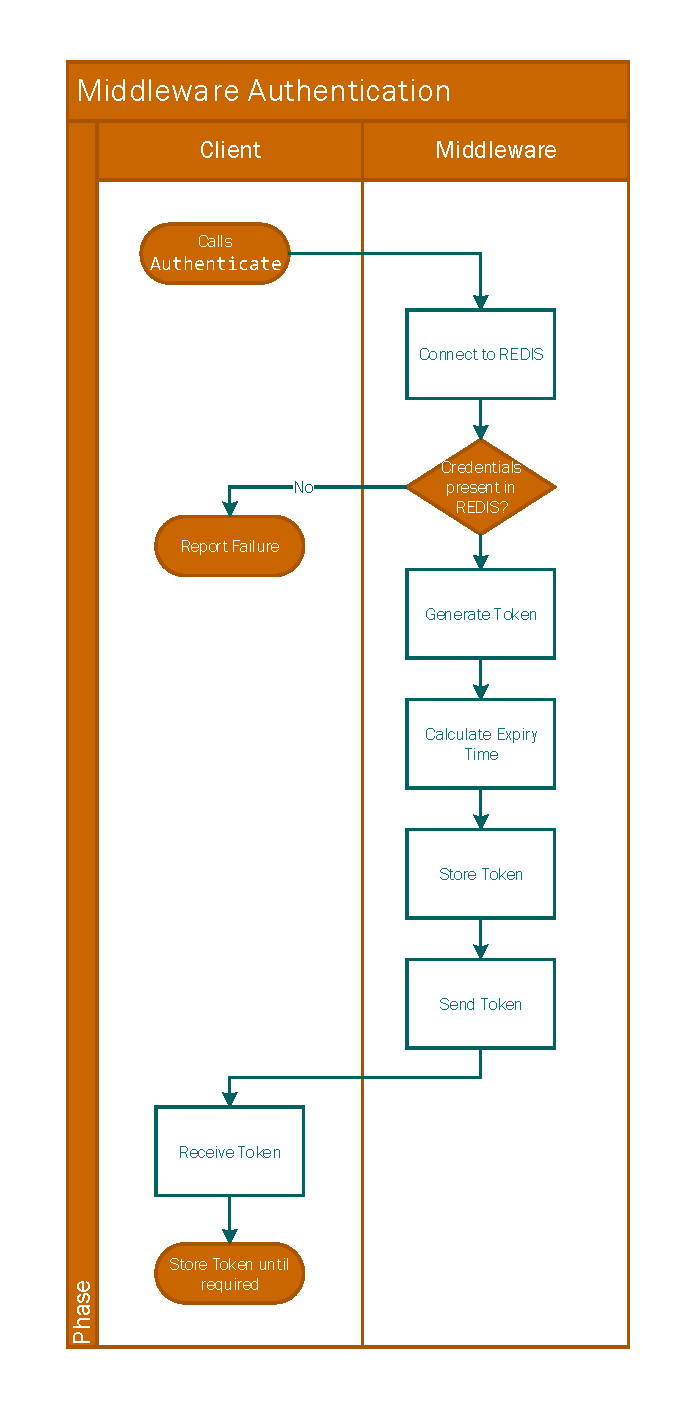
\includegraphics[width=\linewidth]{gfx/MiddlewareAurthentication}} 
\caption{Authentication work-flow}
\label{fig:aurth}
\end{figure}

Once the token has been received successfully the process shown in in \autoref{fig:aurthWithToke} is followed.

 \begin{figure}[!htbp]
\myfloatalign
{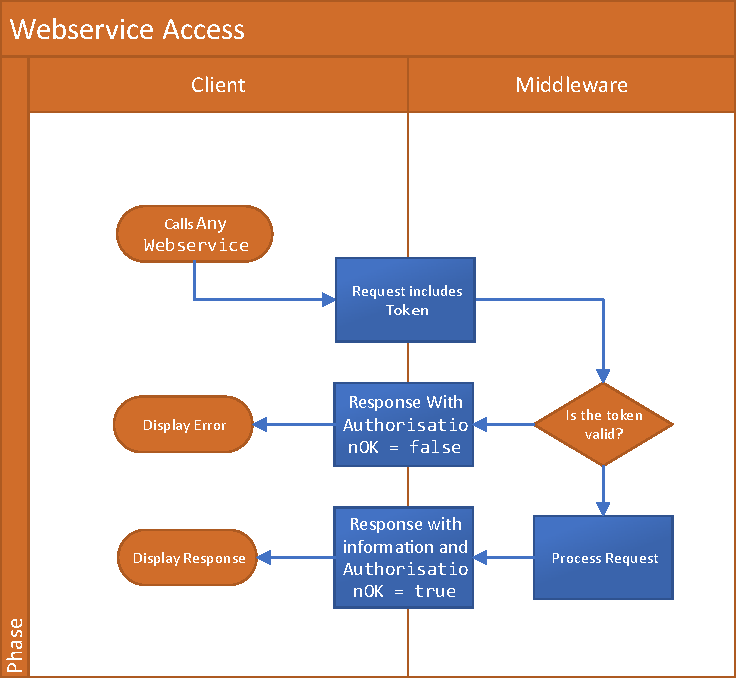
\includegraphics[width=\linewidth]{gfx/MiddlewareAurthenticationWithToken}} 
\caption{Use of authentication token}
\label{fig:aurthWithToke}
\end{figure}

Once the token has been issued to a client it is valid for a fixed amount of time (in the example implementation this is set at one hour, however this is defined as a constant for ease of alteration) after which the client receives an error if it is used. The client must then re-apply for a token, once again using the procedure set out in: \autoref{fig:aurth}. The use of tokens reduces the number of times an end users credentials must be transmitted securely over the network, which would otherwise need to be done with every call to the webservice. Aside from reduced bandwidth usage this scales better on the server-side; the token need simply be checked for validity, rather than recalling the users details and checking the stored password hash.

\vfill
\section{Conclusions}

The case study in the following chapter made extensive use of this middleware and further conclusions are found at the end of that section.

In \autoref{ch:probstate} a number of questions are posed, first amongst them is:

\textit{\QuestionSecurity} 

The middleware is an example of a way to provide security to a datastore with none built in. REDIS, by design, has no security, leaving it to the consuming application for improved speed of data storage and retrieval, which is that project's main focus. When REDIS is hosted on a non publicly accessible server (or port) and accessed via the middleware only authorised users can store or retrieve data. The technique used in the middleware of issuing tokens valid for a limited time has become popular within the industry, though other techniques could also be successfully applied. 

\textit{\QuestionCombine}

Using the middleware as an example we have shown that it is possible to combine multiple data stores by using the same intermediary to connect to all the different datastores. Services run within that intermediary have access to all datastores and thus can perform operations which aggregate data. 

\textit{\QuestionChange}

The use of a cut-out or intermediary between client software and a datastore can safe guard the client application against changes to that datastore or its interfaces. The middleware provides an example of such an application. 

Since the completion of this project Stardog has altered its API and in order as to implement other projects it was necessary to alter the stardog connector module to enable continued operation. Once the stardog connector module had been updated the middleware and the dependant tools continued to operate as before. 

\textit{\QuestionSkillz}

The middleware acts as an intermediary with a known and easily understood interface with external developers. This was used effectively as part of the work presented in \autoref{ch:COMPASS}, where it is assessed.


\section{Further work}

More complete integration of differing data stores is possible - currently there is no webservice to summarise high frequency data and insert the bulk data into another store. This would be easily achieved within the existing framework, however, none of the projects for which the middleware was used have required it, thus it has not been implemented. Before the software could be commercialised it would be necessary to subject it to analysis by penetration testers to find any vulnerabilities in the security mechanism.

\subsection{Outstanding Questions}
\subsubsection{Scalability}
If the middleware is to be deployed at very large scales, handling high frequency sensor at a national or even global scale then scalability challenges will need further examination. 

The middleware is written in a multi-threaded manor, such that it will perform better the more processing cores it has available, however there exists a ceiling beyond which extra hardware will no longer improve performance. The first outstanding challenge is assessing where that ceiling falls and at what scale it would become problematic, if at all. Scalability is already considered within the datastores to which the middleware currently acts as a gateway. Both REDIS and Stardog support clustering, and since the middleware (along with the datastore APIs) are written such that if clustering were deployed with either datastore no changes would be necessary to the middleware. If further performance improvements are found to be necessary then the following changes could be considered:
\begin{itemize}
    \item Deploying multiple servers running the middleware with requests directed to them by a load balancer. This would require minimal alteration to the middleware as it contains no state information. 
    \item The authentication could be handled by an external project designed purely for that purpose, such as \texttt{shiro}\footnote{More details available at: \url{https://shiro.apache.org/}}. This would offer two advantages: 
    \begin{itemize}
        \item Efficiency gains: One performance bottleneck in the middleware is likely to be authentication, this project is dedicated only to providing efficient authentication;
        \item Improved Security: This project has already been heavily tested for security vulnerabilities and is regularly updated whenever they are found.        
    \end{itemize}
    \item Moving to a containerized architecture. This eliminates the overhead of a virtual machine for each deployment of the middleware, in a web-scale, load balanced, environment. Since there is no state preserved in the webservices and WCF webservices can be run in containers, no major issues are foreseen converting to this architecture. 
\end{itemize}

\subsubsection{Datastore Access Speeds}
The two datastores used in this system have very different speed characteristics: REDIS is optimised purely for high frequency data, whilst stardog performs reasoning, which has a performance penalty. Whilst these different speeds were observed over the course of this project they were not measured, nor did this cause any issues. Were services performing combined inserts to be created this synchronisation issue would require further consideration. 
